\section{Lighting}\label{sec:theory_theory_lighting}
Lighting is an important aspect of the game, making it more immersive and has a major impact on how it is perceived by the player.
Artificial light sources present in the game are also indispensable when exploring the world during the in-game night.
In the game, we use three types of light casters: \textit{directional lights}, \textit{point lights}, and \textit{spotlights}.
As the lighting model, we used the \textit{Phong lighting model}.
In this model, light is considered to have 3 components:
\begin{itemize}
    \item ambient lighting $I_a$ (with coefficient $k_a$),
    \item diffuse lighting $I_d$ (with coefficient $k_d$),
    \item specular lighting $I_s$ (with coefficient $k_s$ and material shiness constant $\alpha$).
\end{itemize}
In the case of $N$ light sources in the scene, the total illumination is calculated using the formula
\begin{equation}
    L = k_a I_a + \sum_{i = 1}^N {k_d I_{i, d} \max(0, \langle n, l_i, \rangle) + k_s I_{i, s} \max(0, \langle r_i, v \rangle^\alpha )},
\end{equation}
where $n$ is the normal vector of the fragment, $l$ is the vector pointing from the fragment to the light source, $r$ is the reflection of $l$ on $n$, and $v$ is the vector pointing towards the viewer (all of the aforementioned vectors are assumed to be normalized).
It's important to note that $\langle \cdot, \cdot\rangle$ is the inner product as defined by \autoref{eq:gen-inner-prod}.
The reflected light vector $r$ is calculated using the usual formula
\begin{equation*}
    r = 2 \langle l, n \rangle n - l.
\end{equation*}

\subsection{Directional lighting} \label{subsec:directional-lighting}
During the in-game daytime, the directional light is used to represent the light cast by the sun.
The light direction $l$ is the vector pointing toward the sun.
During the night the directional light is much dimmer but still present.
In this case, the light direction $l$ is pointing toward an imaginary light source ("the stars") which is rotating along with the sky.
\autoref{fig:directional-light} shows the terrain and other game objects illuminated by the directional light of orange color.
\begin{figure}[!htb]
    \centering
    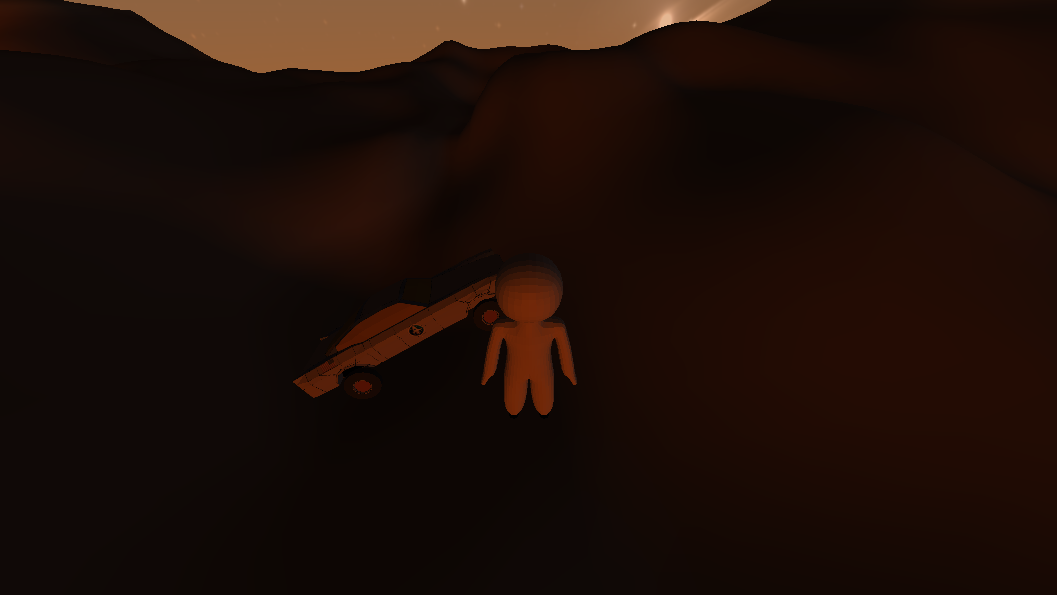
\includegraphics[width=0.8\textwidth]{chapters/theoretical_foundations/sections/lighting/resources/directional-light.png}
    \caption{Directional light}
    \label{fig:directional-light}
\end{figure}
\subsection{Point lights}
In the game, spotlights are represented by white spherical lamps.

In Euclidean geometry, assuming that a point light is placed at a point $p$ and that the current fragment's position is given by $f$, we can calculate the light direction vector $l$ simply as
\begin{equation*}
    l = \frac{p - f}{d_E(p, f)},
\end{equation*}
where $d_E$ is the usual Euclidean distance, i.e.
\begin{equation} \label{eq:dist-euclidean}
    d_E(a, b) = \sqrt{\langle a - b, a - b\rangle_E}.
\end{equation}
For non-Euclidean geometries, we use modified formulas given by \cite{Szirmay-Kalos2022}, namely
\begin{equation}
    l = \frac{p - f \cos(d_S(p, f))}{\sin(d_S(p, f))}
\end{equation}
for spherical geometry and
\begin{equation}
    l = \frac{p - f\cosh(d_H(p, f))}{\sinh(d_H(p, f))}
\end{equation}
for hyperbolic geometry.
The spherical and hyperbolic distances $d_S$ and $d_H$ are given by
\begin{equation} \label{eq:dist-spherical}
    d_S(a, b) = \cos^{-1}(|\langle a, b \rangle_E|)
\end{equation}
and
\begin{equation} \label{eq:dist-hyperbolic}
    d_H(a, b) = \cosh^{-1}(-\langle a, b \rangle_L)
\end{equation}
respectively.

The important difference between a point light and a directional light is the \textit{attenuation} $a$.
Attenuation represents how the light's strength diminishes over distance.
It can be expressed as a reciprocal of a quadratic function:
\begin{equation}
    a = \frac{1}{K_c + K_l d + K_q d^2},
\end{equation}
where $d$ is the distance of the fragment from the source that can be calculated using one of the formulas \ref{eq:dist-euclidean}, \ref{eq:dist-spherical}, or \ref{eq:dist-hyperbolic} depending on the geometry.
Multiplying the light by the attenuation factor gives the desired effect of a realistic point light source such as a lamp, see \autoref{fig:point-lights}.
\begin{figure}[h]
    \centering
    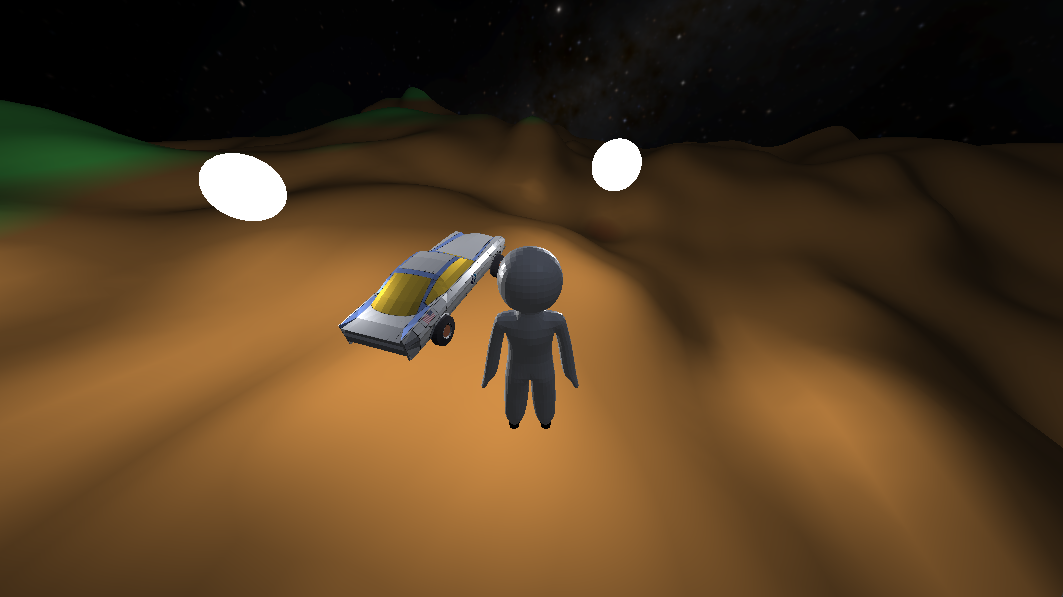
\includegraphics[width=0.8\textwidth]{chapters/theoretical_foundations/sections/lighting/resources/point-lights.png}
    \caption{Point lights}
    \label{fig:point-lights}
\end{figure}
Point lights in hyperbolic and spherical geometry are shown in \autoref{fig:point-light-non-euc}.
\begin{figure*}[h]
    \centering
    \begin{subfigure}[b]{0.475\textwidth}
        \centering
        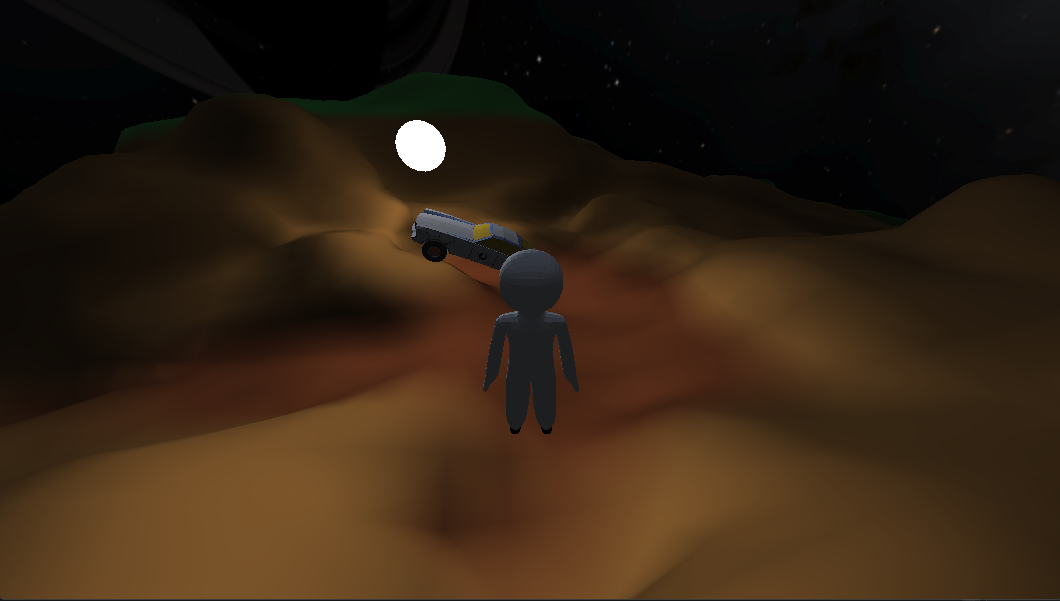
\includegraphics[width=\textwidth]{chapters/theoretical_foundations/sections/lighting/resources/point-light-hyperbolic.png}
        \caption[]%
        {{\small Hyperbolic space}}
        \label{fig:point-light-hyperbolic}
    \end{subfigure}
    \hfill
    \begin{subfigure}[b]{0.475\textwidth}
        \centering
        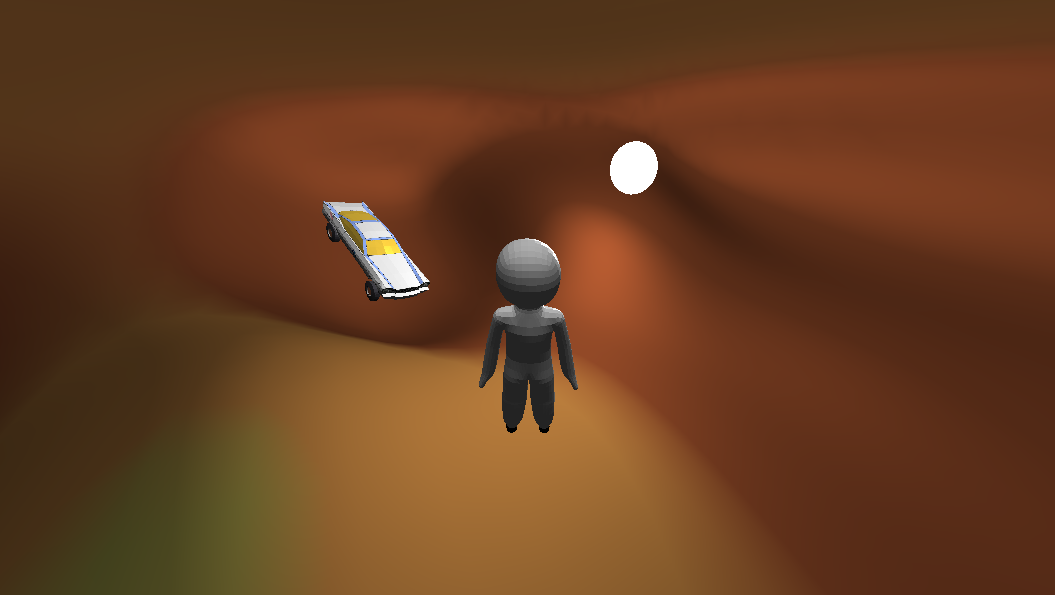
\includegraphics[width=\textwidth]{chapters/theoretical_foundations/sections/lighting/resources/point-light-spherical.png}
        \caption[]%
        {{\small Spherical space}}
        \label{fig:point-light-spherical}
    \end{subfigure}
    \caption[]
    {\small Point lights in non-Euclidean spaces}
    \label{fig:point-light-non-euc}
\end{figure*}
\subsection{Spotlights}
In the game, spotlights are used to represent the player's flashlight and the car's head- and tail lights.

Spotlights are modeled in the same way as point lights, with only one exception.
In the case of spotlights, we want to capture the fact that the light forms a cone.
To do that we calculate the \textit{intensity coefficient} given by
\begin{equation*}
    \mathrm{IC} = \frac{\langle l, -d \rangle - R}{r - R},
\end{equation*}
where $d$ is the vector along which the spotlight is directed, and $R$ and $r$ are the parameters defining the light cone \cite{LearnOpenGL-Light-casters}.
The intensity coefficient is then used to multiply each component of the light, giving the result shown in \autoref{fig:spotlights}.
\begin{figure*}[h]
    \centering
    \begin{subfigure}[b]{0.475\textwidth}
        \centering
        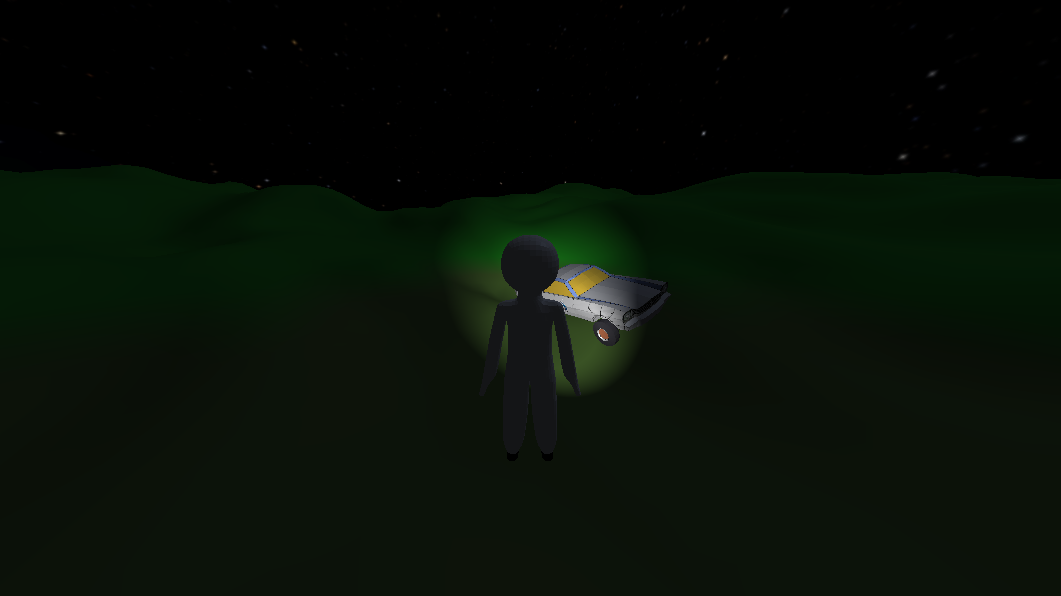
\includegraphics[width=\textwidth]{chapters/theoretical_foundations/sections/lighting/resources/player-flashlight.png}
        \caption[]%
        {{\small Player's flashlight}}
        \label{fig:spotlight-player}
    \end{subfigure}
    \hfill
    \begin{subfigure}[b]{0.475\textwidth}
        \centering
        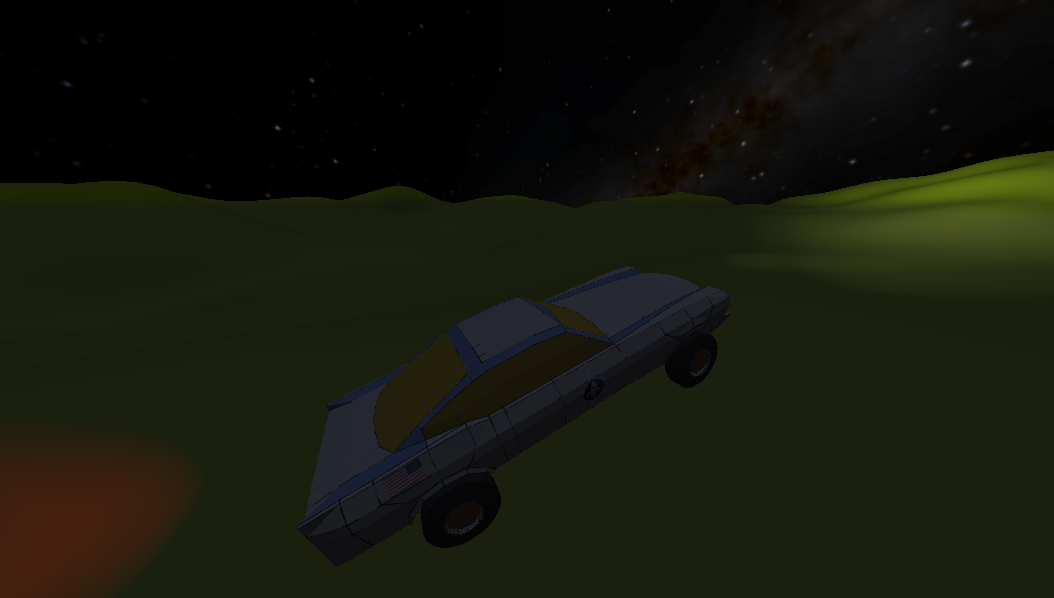
\includegraphics[width=\textwidth]{chapters/theoretical_foundations/sections/lighting/resources/car-lights-spot.png}
        \caption[]%
        {{\small Car illumination}}
        \label{fig:spotlight-car}
    \end{subfigure}
    \caption[]
    {\small Spotlights used in the game}
    \label{fig:spotlights}
\end{figure*}